\section{Deelvraag 4: Requirements}
\label{sec:Requirements}
In dit hoofdstuk word de vierde deelvraag onderzocht \textit{\SubquestionFour}
Om met deze deelvraag te beantwoorden zijn er semi gestructureerde interviews gehouden met de product owner en de CEO van Snakeware.
Tijdens de interviews wordt er gepraat over de eisen en wensen zodat deze in kaart kunnen worden gebracht.
Beide interviews zijn terug te vinden in bijlage \ref{appendix:ExploreUserRequirements}.

\subsection{Interview met Elsa Croes en Eric Dijkstra}
Het eerste interview wat plaats heeft gevonden is gedaan met de product owner Elsa Croes.
Om Elsa te ondersteunen en meer technisch kennis mee te nemen in het interview is er op het laatst moment een frontend developer mee genomen in het gesprek Eric Dijkstra.
Het interview heeft plaats gevonden op 6 november 2023 op locatie bij Snakeware.
Het interview begon met een kleine introductie wie ze zijn en wat ze doen binnen Snakeware.
Daarna zijn er eerst vragen gesteld om de kern functionaliteiten in beeld te krijgen en de eisen en wensen van de product owner.
Hier is er gesproken over een toekomstvisie van het systeem en de mogelijke functionaliteiten die zouden toegevoegd kunnen worden.

\whitespace
Er is ook gesproken over het belang van SEO in het proof of concept en hoe belangrijk dat dit geimplementeerd wordt.
Elsa en Eric gaven beide aan dat SEO erg belangrijk is voor een moderne site.
Zonder SEO-opties zou een site niet gebruikt kunnen worden klanten omdat ze dan niet goed gevonden kunnen worden.
Het complete interview is te vinden in bijlage \ref{appendix:ExploreUserRequirementsElsa}.

\subsection{Interview Hans Hoomans}
Daarnaast is er ook interview gedaan met de CEO van Snakeware Hans Hoomans.
Het interview heeft plaats gevonden op 7 november 2023 op locatie bij Snakeware.
Tijdens het interview is erg van het originele pad afgegaan van de originele geplande vragen.
Er is vooral gesproken over een nieuw mogelijk datamodel en hoe dat impact zou hebben op het totale systeem.

\whitespace
Daarnaast is het een belangrijk voor Hans dat het PoC niet rigide aanvoelt.
Hans geeft aan dat een van de problemen waar Snakeware nu vaak tegen aanloopt, is dat er vaak een custom oplossing moet komen voor alle verschillende klante.
Hij wilt graag dat er meer generiek gewerkt binnen Snakeware en dat software vaker hergebruikt kan worden. 
De quote waar Hans graag naar toe wilt streven is \qw{kracht van eenvoud en herhaling}.
Dit zou hij graag terug willen zien in het datamodel door minder tabellen te gebruiken en meer generiek te werken.
Tijdens het interview is er informatie besproken dat hans liever niet in de transcriptie wilt hebben.
Hierom wordt er een samenvatting gemaakt van het interview deze samenvatting is te vinden in bijlage \ref{appendix:ExploreUserRequirementsHans}
% Aan het einde van het interview zijn we de vragen nog een keer langs gelopen en hebben we hier uit verschillende requirements gehaald.
% Omdat dit interview niet als transcriptie gebruikt kan worden is er een samenvatting gemaakt en is te vinden in bijlage \ref{appendix:ExploreUserRequirementsHans}.
%


% \subsection{Interviews met sleutelfiguren}
% Het eerste interview wat plaats heeft gevonden is gedaan met de product owner Elsa Croes.
% Om Elsa te ondersteunen en meer technisch kennis mee te nemen in het interview is er op het laatst moment een frontend developer mee genomen in het gesprek Eric Dijkstra.
% Het interview heeft plaats gevonden op 6 november 2023 op locatie bij Snakeware.
% Tijdens het interview zijn er verschillende vragen gesteld om een beeld te krijgen van de toekomstvisie van de applicatie.
% Het complete interview is te vinden in bijlage \ref{appendix:ExploreUserRequirementsElsa}.
%
% \whitespace
% Daarnaast is er ook interview gedaan met de CEO van Snakeware Hans Hoomans.
% Het interview heeft plaats gevonden op 7 november 2023 op locatie bij Snakeware.
% Tijdens het interview met Hans zijn we heel erg van de originele vragen afgegaan. 
% Aan het einde van het interview zijn we de vragen nog een keer langs gelopen en hebben we hier uit verschillende requirements gehaald.
% Omdat dit interview niet als transcriptie gebruikt kan worden is er een samenvatting gemaakt en is te vinden in bijlage \ref{appendix:ExploreUserRequirementsHans}.
%
% De complete lijst met de requirements die uit dit interview zijn te zien in \ref{fig:ElsaRequirements}.
%
% \whitespace
% \begin{graphic}
%     \captionsetup{type=figure}
%     \caption{Elsa Croes Requirements}
%     
\includegraphics[scale=0.2]{Placeholder.jpg}
%     \label{fig:ElsaRequirements}
% \end{graphic}

\subsection{Antwoord en resultaat}
Na dat beide interviews waren afgenomen is er een lijst van user stories gemaakt.
Deze user stories zijn beide door Hans en Elsa als correct beschouwd.
In figuur \ref{fig:RequirementSimplified} zij de requirements te vinden.

% Het andere interview is gedaan met de CEO van Snakeware Hans Hoomans.
% De complete transcriptie van het interview is te vinden in bijlage \ref{appendix:ExploreUserRequirementsHans}
% Het interview heeft plaats gevonden op 7 november 2023 op locatie.
%
\begin{graphic}
    \captionsetup{type=figure}
    \caption{Resultaat user requirements exploration}
    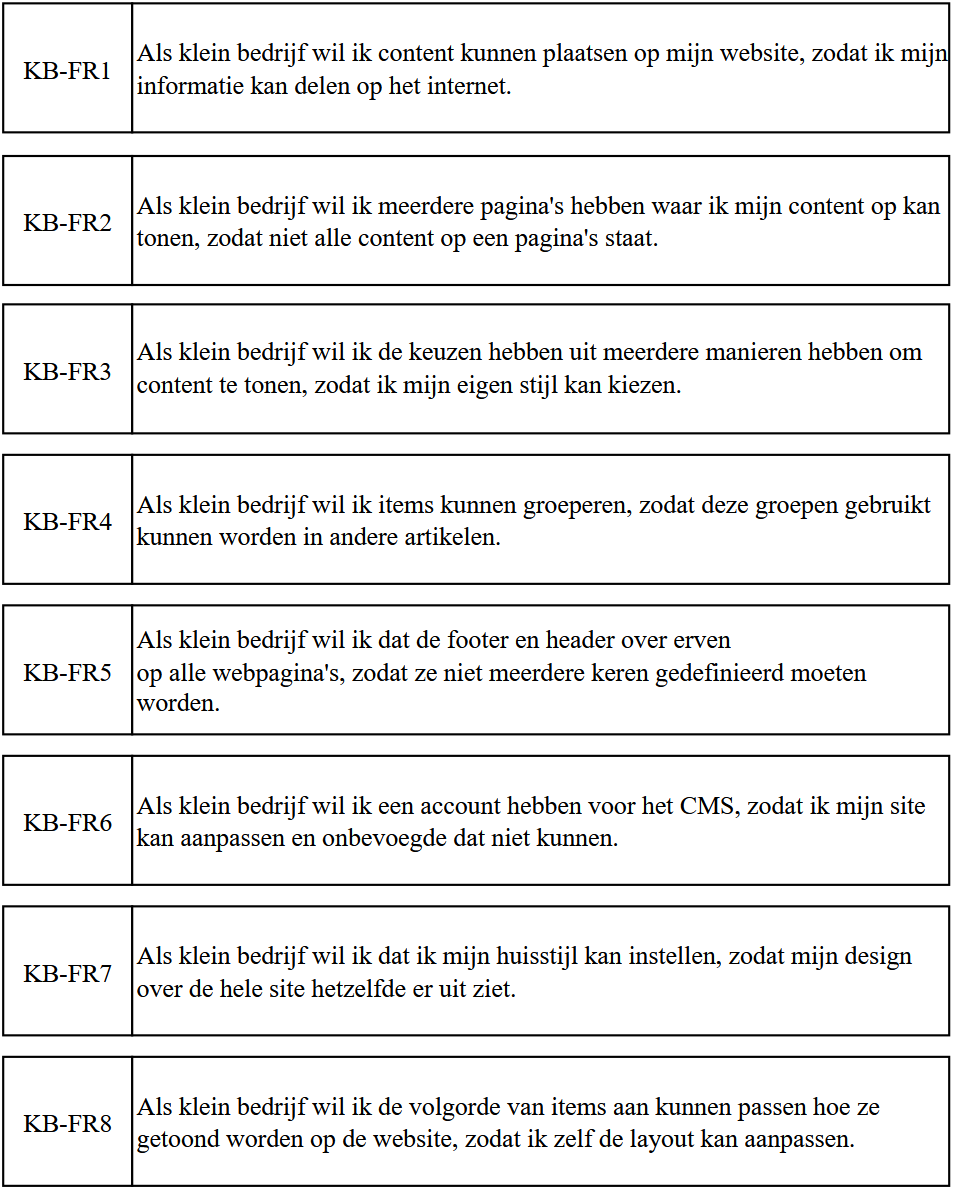
\includegraphics[scale=0.4]{FR1-8}

    \whitespace
    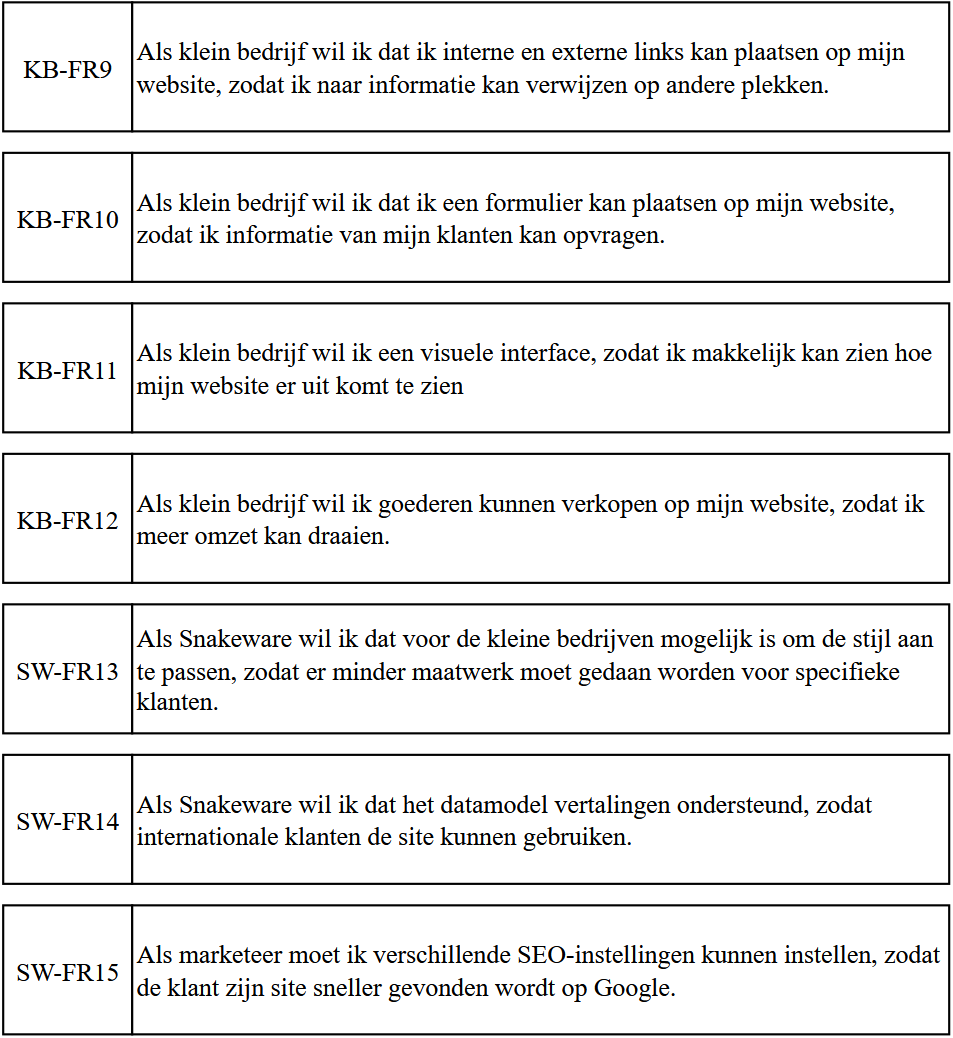
\includegraphics[scale=0.4]{FR9-15}
    \label{fig:RequirementSimplified}
\end{graphic}
